%implementing document formatting:
%page setup (page size, text size, page layout, chapters start on a new page).
%memoir is a form of book class that supports any kind of document.
\documentclass[fleqn,a4paper,12pt,twoside,openany]{memoir}

%setting the header and footer in that order:
\setheadfoot{28pt}{28pt} %if any problems are encountered, try changing the latter 28pt with 1cm.

%setting language:
\RequirePackage[danish, english]{babel}

%this package makes it possible to treat any element as a float,
%figures and tables are by default treated as floats.
%read http://en.wikibooks.org/wiki/LaTeX/Floats,_Figures_and_Captions to specify your float.
\usepackage{float}
\usepackage{wrapfig}
\usepackage{placeins}

%this package makes it possible to make theorems and examples:
\usepackage{amsthm}
%setting the style of examples (parameters: plain, definition, remark):
%(definition is usually used for examples)
\theoremstyle{definition}
%the frist parameter is the syntax used in the document, the second is that which is printed in LaTex.
\newtheorem{example}{Eksempel}

%making it possible to use æ, ø and å:
\usepackage[utf8]{inputenc}
%helps with word division when using æ, ø and å, and makes it ps-font rather than bmp:
\usepackage[T1]{fontenc}

%package for implementation of graphic files:
\usepackage{graphicx}

%package for captions
\usepackage[nooneline]{caption}

%%package for implementation of math:
\usepackage{amsmath , amsfonts , amssymb, float}

%allowing use of color:
\usepackage{color}
%allowing use of more colors also in tables (see: http://en.wikibooks.org/wiki/LaTeX/Colors):
\usepackage[usenames,dvipsnames,svgnames,table]{xcolor}

%hyperlinks in the tabel of contents - comment this out before the report is printed.
\usepackage{hyperref}
\hypersetup{
%	bookmarks = true,  % Show 'bookmark'-frame in pdf.
	colorlinks = true, % True = colored links, False = framed links.
	citecolor = blue,  % Link color for references.
	linkcolor = blue,  % Link color in table of contents.
	urlcolor = blue,   % Link color for extern URLs.
}

%makes it possible to refer to the name of a chapter rather than just the number.
\usepackage{nameref}

%package for the SI unit standard
\usepackage{siunitx}

%package for writing program code in latex
\usepackage{listings}

\lstset{ 
language=C,               	 	% choose the language of the code
basicstyle=\footnotesize,       % the size of the fonts that are used for the code
numbers=left,                   % where to put the line-numbers
numberstyle=\footnotesize,      % the size of the fonts that are used for the line-numbers
stepnumber=1,                   % the step between two line-numbers. If it is 1 each line will be numbered
numbersep=5pt,                  % how far the line-numbers are from the code
backgroundcolor=\color{white},  % choose the background color. You must add \usepackage{color}
showspaces=false,               % show spaces adding particular underscores
showstringspaces=false,         % underline spaces within strings
showtabs=false,                 % show tabs within strings adding particular underscores
frame=single,           		% adds a frame around the code
tabsize=2,          			% sets default tabsize to 2 spaces
captionpos=b,           		% sets the caption-position to bottom
breaklines=true,       			% sets automatic line breaking
breakatwhitespace=false,    	% sets if automatic breaks should only happen at whitespace
escapeinside={\%*}{*)}          % if you want to add a comment within your code
}

%setting references (using numbers) and supporting i.a. Chicargo-style:
\usepackage{etex}
\usepackage{etoolbox}
\usepackage{keyval}
\usepackage{ifthen}
\usepackage{url}
\usepackage{csquotes}
\usepackage[backend=biber,url=true,doi=true,style=numeric, sorting=none]{biblatex}
\bibliography{bibliography/bibliography.bib}

%this package makes it possible include pdf pages in fx appendix;
%using  following syntax: \includepdf[pages={1}]{myfile.pdf}
\usepackage{pdfpages}

%%%MARGINER%%%
\setlrmarginsandblock{3.5cm}{2.5cm}{*}	% \setlrmarginsandblock{inner margin}{outer margin}{ratio}
\setulmarginsandblock{2.5cm}{3.0cm}{*}	% \setulmarginsandblock{top}{bottom}{ratio}
\checkandfixthelayout 			            % fixes stuff..

%Enables the use FiXme refferences. Syntax: \fxnote{...}
%With "final" in stead of "draft" an error will ocure for every FiXme
%under compilation.
\usepackage[footnote,draft,english,silent,nomargin]{fixme}

%%%CHAPTERLAYOUT%%%
%setting the color of the chapter number
\definecolor{numbercolor}{gray}{0.7}
%Downloaded chapter-setup:
\newif\ifchapternonum
\makechapterstyle{jenor}{
  \renewcommand\printchaptername{}
  \renewcommand\printchapternum{}
  \renewcommand\printchapternonum{\chapternonumtrue}
  \renewcommand\chaptitlefont{\fontfamily{pbk}\fontseries{db}\fontshape{n}\fontsize{25}{35}\selectfont\raggedleft}
  \renewcommand\chapnumfont{\fontfamily{pbk}\fontseries{m}\fontshape{n}\fontsize{1in}{0in}\selectfont\color{numbercolor}}
  \renewcommand\printchaptertitle[1]{%
    \noindent
    \ifchapternonum
    \begin{tabularx}{\textwidth}{X}
    {\let\\\newline\chaptitlefont ##1\par} 
    \end{tabularx}
    \par\vskip-2.5mm\hrule
    \else
    \begin{tabularx}{\textwidth}{Xl}
    {\parbox[b]{\linewidth}{\chaptitlefont ##1}} & \raisebox{-15pt}{\chapnumfont \thechapter}
    \end{tabularx}
    \par\vskip2mm\hrule
    \fi
  }
}
%setting chapter style:
\chapterstyle{jenor}

\usepackage{textpos}

%depth of numbered headlines (part/chapter/section/subsection):
\setsecnumdepth{none}
\maxsecnumdepth{none}
%depth of the table of contents:
\settocdepth{section}

% Makes sure LaTeX does not stretch the text at page break:
\raggedbottom
%Figure references:
\newcommand{\figref}[1]{\textbf{figure \ref{#1}}}

%Figure references after full stop/period:
\newcommand{\Figref}[1]{\textbf{Figure \ref{#1}}}

%Table references:
\newcommand{\tableref}[1]{\textbf{table \ref{#1}}}

%Table references after full stop/period:
\newcommand{\Tableref}[1]{\textbf{Table \ref{#1}}}

%Units:
\newcommand{\unit}[1]{&& \left[\si{#1}\right]}

%Text:
\newcommand{\tx}[1]{\text{#1}}

%Equation references:
%1 equation:
\renewcommand{\eqref}[1]{\textbf{equation (\ref{#1})}}
%2 equations:
\newcommand{\eqrefTwo}[2]{\textbf{equation (\ref{#1})} and \textbf{(\ref{#2})}}
%3 equations:
\newcommand{\eqrefThree}[3]{\textbf{equation (\ref{#1})}, \textbf{(\ref{#2})} and \textbf{(\ref{#3})}}
%4 equations:
\newcommand{\eqrefFour}[4]{\textbf{equation (\ref{#1})}, \textbf{(\ref{#2})}, \textbf{(\ref{#3})} and \textbf{(\ref{#4})}}
%5 equations:
\newcommand{\eqrefFive}[5]{\textbf{equation (\ref{#1})}, \textbf{(\ref{#2})}, \textbf{(\ref{#3})}, \textbf{(\ref{#4})} and \textbf{(\ref{#5})}}
%5 equations:
\newcommand{\eqrefSix}[6]{\textbf{equation (\ref{#1})}, \textbf{(\ref{#2})}, \textbf{(\ref{#3})}, \textbf{(\ref{#4})}, \textbf{(\ref{#5})} and \textbf{(\ref{#6})}}
%5 equations:
\newcommand{\eqrefSeven}[7]{\textbf{equation (\ref{#1})}, \textbf{(\ref{#2})}, \textbf{(\ref{#3})}, \textbf{(\ref{#4})}, \textbf{(\ref{#5})}, \textbf{(\ref{#6})} and \textbf{(\ref{#7})}}

%Equation references after full stop/period:
%1 equation:
\newcommand{\Eqref}[1]{\textbf{Equation (\ref{#1})}}
%2 equations:
\newcommand{\EqrefTwo}[2]{\textbf{Equation (\ref{#1})} and \textbf{(\ref{#2})}}
%3 equations:
\newcommand{\EqrefThree}[3]{\textbf{Equation (\ref{#1})}, \textbf{(\ref{#2})} and \textbf{(\ref{#3})}}
%4 equations:
\newcommand{\EqrefFour}[4]{\textbf{Equation (\ref{#1})}, \textbf{(\ref{#2})}, \textbf{(\ref{#3})} and \textbf{(\ref{#4})}}
%5 equations:
\newcommand{\EqrefFive}[5]{\textbf{Equation (\ref{#1})}, \textbf{(\ref{#2})}, \textbf{(\ref{#3})}, \textbf{(\ref{#4})} and \textbf{(\ref{#5})}}
%5 equations:
\newcommand{\EqrefSix}[6]{\textbf{Equation (\ref{#1})}, \textbf{(\ref{#2})}, \textbf{(\ref{#3})}, \textbf{(\ref{#4})}, \textbf{(\ref{#5})} and \textbf{(\ref{#6})}}
%5 equations:
\newcommand{\EqrefSeven}[7]{\textbf{Equation (\ref{#1})}, \textbf{(\ref{#2})}, \textbf{(\ref{#3})}, \textbf{(\ref{#4})}, \textbf{(\ref{#5})}, \textbf{(\ref{#6})} and \textbf{(\ref{#7})}}
\begin{document}

%||||||||||||||||||||||||||||||||||||||||||||||||||||||||||||||||
%|||||||                 Example Inputs                  ||||||||
%||||||||||||||||||||||||||||||||||||||||||||||||||||||||||||||||
%|||||||                                                 ||||||||
%             \section{Figure Sample}

\begin{figure}[H]
	\caption{CAPTION\fxnote{Remember source}}
	\label{LABEL}
	\centering
	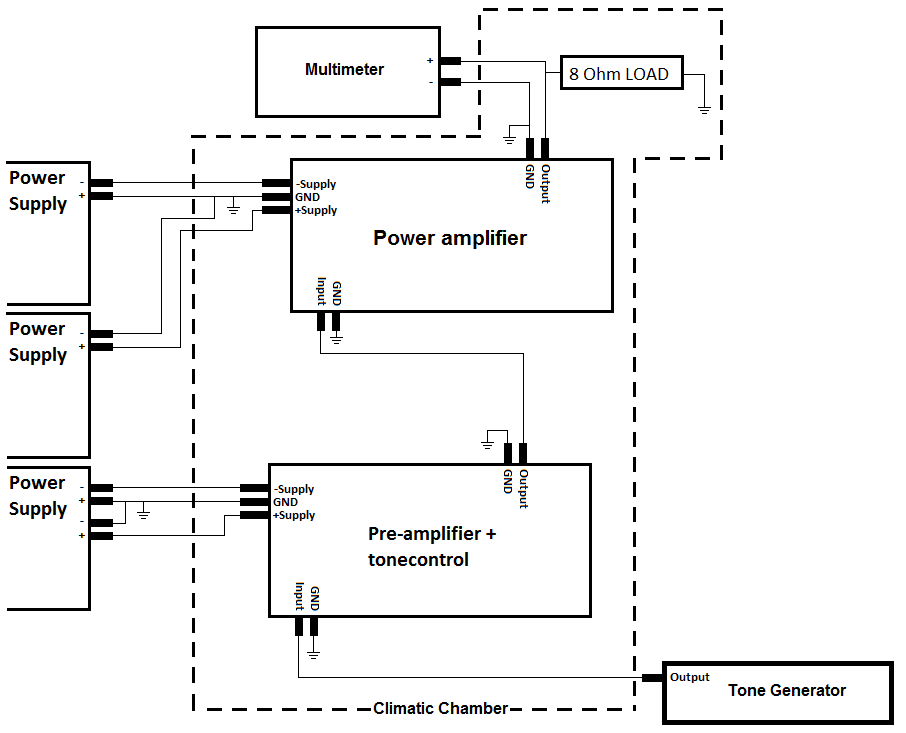
\includegraphics[scale=.6]{figures/filename}
	\flushleft
	\textit{SOURCE}
\end{figure}

%--------- NOTES ------------------------------------------------------
%Fxnotes wont compile properly inside the figure, only in the caption.
%Filetype ([...]{figures/filename.jpg}) can be specified but isn't needed.

\figref{LABEL} \Figref{LABEL}

%Do not use \vspace{length} or \hspace{length} or \noindent etc unless exceedingly necessary - LaTeX is a markup language, let it do its job.
\vspace{.5cm}
\noindent
%--------- BIBLIOGRAPHY REF EKSAMPLE -----------------------------------
This reference only represents this line since it is before the punctuation mark\cite{YDing}. This next reference however represents the entire section. That is all of the preceding sentences in the entire section. This is due to the fact that it is now after the punctuation mark in the end of the section (this is not used in the middle of a section!).\cite{YDing}
%>>>>>>>>>>>>>>>PLEASE ALSO READ THE NOTE IN bibliography/bibliography.bib<<<<<<<<<<<<<<<<<<
\pagebreak         %|||||||
%             \section{Table Sample}

\begin{table}[H]
\caption{This Is a Table\label{LABEL}}
\begin{tabular}{|l|p{5cm}|l|l|l|}
  \hline %-----------------------------------------------------------------------------------
  \textbf{No.} &\textbf{Description} &\textbf{Min} &\textbf{Max} &\textbf{Requirements}    \\
  \hline %-----------------------------------------------------------------------------------
  1            & Some Text           & Some Text   & Some Text   & Some Text               \\
               &                     &             &             & Some More Text          \\
               &                     &             &             & Text Text               \\
               &                     &             &             & Text Text Text          \\
  \hline %-----------------------------------------------------------------------------------
  2            & Some Text           & Some Text   & Some Text   & Some Text               \\
  \hline %-----------------------------------------------------------------------------------
  3            & By specifying the
                 width of a column
                 (|p\{5cm\}|) the
                 cells in that column
                 will not exceed the
                 specified width but         %Extra hitespaces is used only for clarity
                 instead expand              %and will not affect the compiled output.
                 downward.
                                     & Some Text           & Some Text   & Some Text       \\
  \hline %-----------------------------------------------------------------------------------
  4            & Some Text           & Some Text   & Some Text   & Some Text               \\
  \hline %-----------------------------------------------------------------------------------
  \multicolumn{2}{|l|}{Some Text}    & \multicolumn{3}{l|}{Some Text}                      \\
  \hline %-----------------------------------------------------------------------------------
  \multicolumn{2}{|l|}{Text Text}    & \multicolumn{3}{l|}{Text = Text}                    \\
  \multicolumn{2}{|l|}{}             & \multicolumn{3}{l|}{Text = Text}                    \\
  \multicolumn{2}{|l|}{}             & \multicolumn{3}{l|}{Text = Text}                    \\
  \multicolumn{2}{|l|}{}             & \multicolumn{3}{l|}{Text = Text}                    \\
  \multicolumn{2}{|l|}{}             & \multicolumn{3}{l|}{Text = Text}                    \\
  \hline %-----------------------------------------------------------------------------------
  \multicolumn{2}{|l|}{Some Text}    & \multicolumn{3}{l|}{Teeeexxtt}                      \\
  \multicolumn{2}{|l|}{}             & \multicolumn{3}{l|}{\LaTeX}                         \\
  \hline %-----------------------------------------------------------------------------------
\end{tabular}
\end{table}

\tableref{LABEL} \Tableref{LABEL}

\pagebreak          %|||||||
%             \section{Equation Sample}

Ohms Law:
\begin{flalign}
  U &= I \times R \unit{\volt}
  \label{eq1}
\end{flalign}
%
Some explanation:
\begin{flalign}
  [Equation] &= [Number] \unit{Unit}
  \label{eq2}
\end{flalign}
%
Some explanation:
\begin{flalign}
  [Equation] &= [Number] \unit{Unit}
  \label{eq3}
\end{flalign}
%
Some explanation:
\begin{flalign}
  [Equation] &= [Number] \unit{Unit}
  \label{eq4}
\end{flalign}
%
Some explanation:
\begin{flalign}
  [Short Equation] &= [Number] \unit{Unit}
  \label{eq5}\\ %<-------------------------------------------------| Remember linebreak AFTER
  [Somewhat Longer Equation] &= [Number] \unit{Unit} %             | label when writing multiple
  \label{eq6}\\ %<-------------------------------------------------| equations.
  [Somewhat Quite a Lot Longer Equation] &= [Number] \unit{Unit}
  \label{eq7}
\end{flalign}
%
%
\eqref{eq1}\\
%
\eqrefTwo{eq1}{eq2}\\
%
\eqrefThree{eq1}{eq2}{eq3}\\
%
\eqrefFour{eq1}{eq2}{eq3}{eq4}\\
%
\eqrefFive{eq1}{eq2}{eq3}{eq4}{eq5}\\
%
\eqrefSix{eq1}{eq2}{eq3}{eq4}{eq5}{eq6}\\
%
\eqrefSeven{eq1}{eq2}{eq3}{eq4}{eq5}{eq6}{eq7}\\
%
\Eqref{eq1}\\
%
\EqrefTwo{eq1}{eq2}\\
%
\EqrefThree{eq1}{eq2}{eq3}\\
%
\EqrefFour{eq1}{eq2}{eq3}{eq4}\\
%
\EqrefFive{eq1}{eq2}{eq3}{eq4}{eq5}\\
%
\EqrefSix{eq1}{eq2}{eq3}{eq4}{eq5}{eq6}\\
%
\EqrefSeven{eq1}{eq2}{eq3}{eq4}{eq5}{eq6}{eq7}
%
\pagebreak       %|||||||
             \chapter{Test Title} %\label{put a label here and uncomment}
\textbf{Name: Group 510}\\
\textbf{Date: ??/?? - 2015}

\section*{Purpose}
The purpose of the module test. If testing specifications, include these here.
\\

\section*{Setup}
Input a diagram of the test setup:
%\begin{figure}[H]
%	\centering
%	\includegraphics[scale=.6]{figures/figureNameHere}
%	\flushleft
%	\caption{Test setup for ...}
%\end{figure}

\section*{List of Equipment}
Example of list of equipment:
\begin{table}[H]
\begin{tabular}{|l|l|p{4cm}|}
\hline%-------------------------------------------------------------------
  \textbf{Instrument}           &  \textbf{AAU-no.}  &  \textbf{Type}    \\
\hline%-------------------------------------------------------------------
  Oscilloscope                  &  52773             &  Agilent 54621D  \\
\hline%-------------------------------------------------------------------
  FPGA							&                    &   Spartan-3 (Chip:xc3s1000)  \\
\hline%-------------------------------------------------------------------
  Laptop                        & 	                 &       \\
\hline%-------------------------------------------------------------------
\end{tabular}\\
\end{table}

\section*{Procedure}

\begin{enumerate}
\item write each step as done after setup - if there are different configurations of setup remember to include these.
\end{enumerate}

\section*{Results}

Example of results:
\begin{table}[H]
\begin{tabular}{|l|l|l|l|}

\hline%------------------------------------------------------------------------------------------------------
           & \textbf{Expected Result}   & \textbf{Result} \\
\hline%------------------------------------------------------------------------------------------------------
  \textit{Frequency}           &  49.5 - 50.5 $Hz$ &  50 $Hz$  \\
\hline%------------------------------------------------------------------------------------------------------
\textit{Ammplitude}                     &   3.1 - 3.4 $V$            &    3.3 $V$          \\
\hline%------------------------------------------------------------------------------------------------------
 \textit{Pulse Width: Min}     &    5 \% (1 $ms$)          &     1  $ms$   \\
\hline%------------------------------------------------------------------------------------------------------
\textit{Pulse Width: Med}      &      7.5 \% (1.5 $ms$)           & 1.5 $ms$            \\
\hline%------------------------------------------------------------------------------------------------------
  \textit{Pulse Width: Max}   &    10 \% (2 $ms$)             &  2 $ms$         \\
\hline%------------------------------------------------------------------------------------------------------

\end{tabular}
\end{table}         %|||||||
%|||||||                                                 ||||||||
%||||||||||||||||||||||||||||||||||||||||||||||||||||||||||||||||
%||||||||||||||||||||||||||||||||||||||||||||||||||||||||||||||||


%---------------------------INPUTS-------------------------------


\part{Design \& implementation}
\chapter{Design Consideration}
In this chapter the system will be designed with a top-down approach. First a use-case of the overall functionalities in the system is described, in order to give an overall view of what the system must be able to do. Furthermore ..  

\section{Use case design}
To give an overall view of what the system should be able to do, a UML use-case diagram is used to consider and describe the main functionalities and operators in the system, see \figref{fig:usecase}.

 \begin{figure}[H]
	\centering
	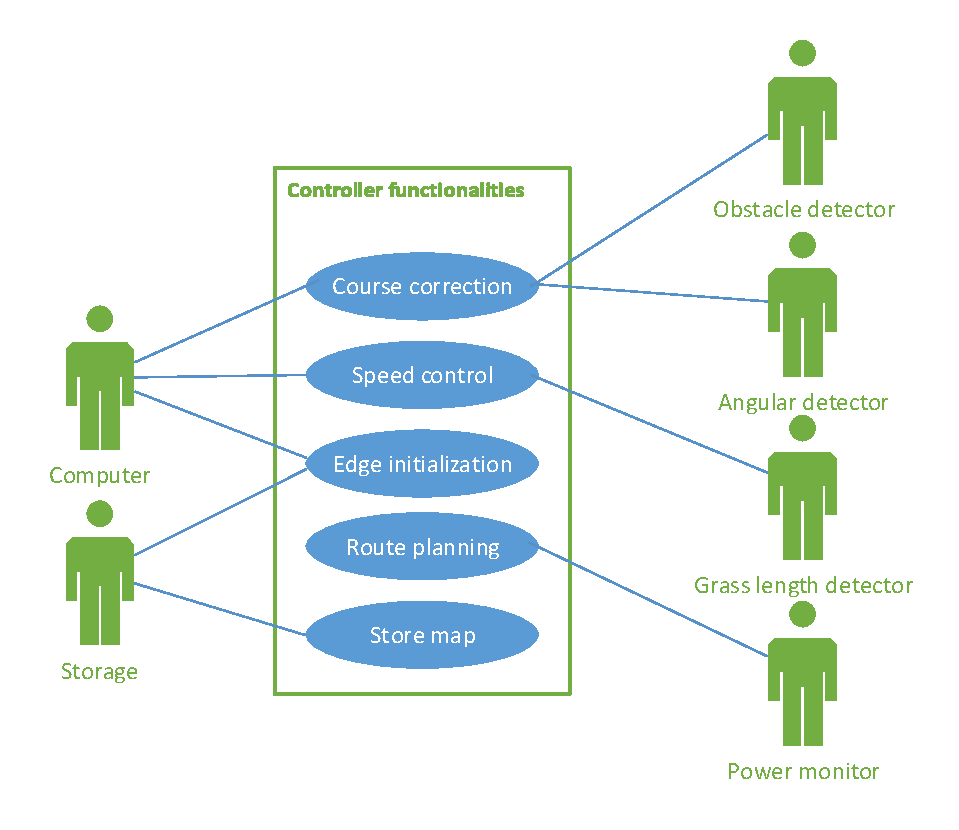
\includegraphics[scale=0.9]{figures/P5UseCase.pdf}
	\caption{Use-Case Diagram}
	\label{fig:usecase}
	\flushleft
\end{figure}

\noindent
The main purpose of the system is to automatically navigate in a specific area. In which area to navigate is decided by the \textit{Edge initialization} functionality, which uses the \textit{Store map} functionality to store the information in storage.\\\\
The route to navigate, in the specific area, is provided by the functionality \textit{Route planning}. \textit{Route planning} uses the information, about the specific area, provided by \textit{Edge initialization} to plan the most optimal route in which to follow. Furthermore the \textit{Route planning} needs information about the systems power level to insure the \textit{Route planning} takes into consideration if the system needs charging.\\\\
To insure the system is moving with a constant speed or a speed which is fitted to the height of the grass, detected with the \textit{Grass length detector}, a \textit{Speed control} functionality is necessary in the system.\\\\
The last functionality, \textit{Course correction},  

include rain sensor

 


 
 
\section{The Games on Track GT-position system}
Header\\\\
The Games on Track GT-Position system, shortened GoT, is a GPS system which uses radio-waves and ultrasound to locate the object. The system is build up by three hardware components, the transmitter, receiver and master. 

\subsubsection{Transmitter}
The transmitter component is placed on the object, which needs to be located. To indicate the objects position, the transmitters emits out ultrasound waves to indicate where it and the object is positioned. The transmitter component runs on 2 AA-batteries and therefore does not need an external power-source. 

\subsubsection{Receiver}
\fxnote{What kind of "radio waves" does the receiver transmit data to the master?}
The receiver component is placed around the area where the object, with the transmitter, has to be located. The receivers assignment is to search for the ultrasound waves, which the transmitter is emitting. The ultrasound waves received by the receivers, provides information containing the distance between the specific receiver to the transmitter located on the object. To be able to calculate the exact position of the transmitter and the object, a minimum of three receivers is necessary. however, more receivers can be added to the system for more reliability and the ability to cover a larger area. For the receivers to work at a high efficiency, they should be placed 1 to 2 meters apart and not on a single line (See \figref{receiverSetup}). But if receivers shall cover a bigger area, they can be placed up to a distance of 5 meters between them, however, this would affect the measurement and thereby make it less reliable. The receivers have a maximum reach of 8 meters. The receivers needs between 14 to 20 volt DC. Thus, making the receivers able to be powered through a computer charger if necessary.

\begin{figure}[H]
	\centering
	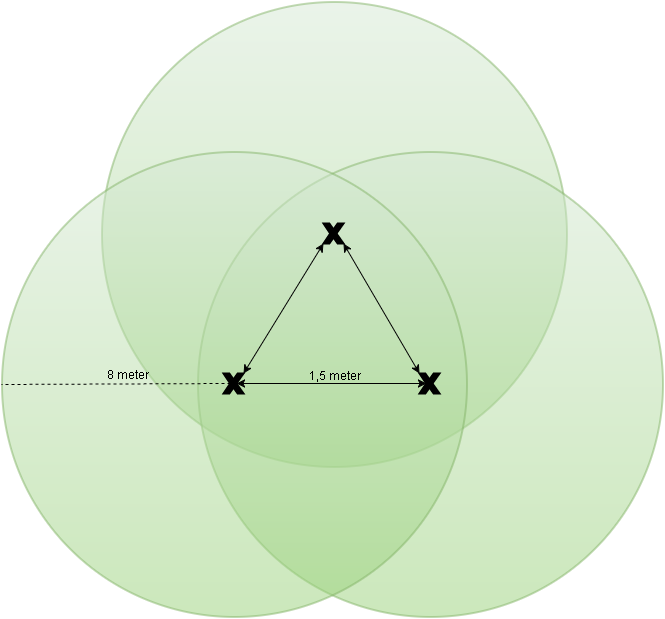
\includegraphics[scale=0.5]{figures/ReceiverSetup.png}
	\caption{Example on a standard setup for the receivers. \fxnote{increase size of text in figure}}
	\label{receiverSetup}
	\flushleft
\end{figure}

\subsubsection{Master}
The master is a receiver which should be connected to a computer. The masters assignment is to receive the data transmitted from the individual receivers and send it directly to the connected computer. The master is powered through a USB cable, between the master and the computer.\\\\

\subsubsection{Computer}
The program on the computer, which handles the information received from the master, uses the data to calculate the position of the transmitter. This is done with a method call Trilateration. Trilateration is a way of calculating a position, in a three-dimensional space, from three distances (from known locations), with the help of spheres, circles and triangles. Therefore it is necessary for the system to have atleast three receivers, as mentioned earlier.  With additional receivers a check up can be performed to ensure the position of the transmitter is correct.Trilateration does not work, if the three know points is on a single line and therefore shall the receivers be placed in a triangle.\\\\

If the receivers have been moved, it is necessary to calibrate the system. This is done with a calibration triangle. The calibration triangle is made of three points on a flat surface and have a distance of 40 to 200 centimeters between them. One of the points on the calibration triangle is made the origin (0,0,0) of the new coordinate system. Another point on the triangle will then be call (X,0,0), in which the line between the first point and the second point will become the X-axis. The last point will be call (X,Y,0) and will determine in which way the positive Y-axis will go. The surface which the calibration triangle is placed on, will be the XY-plan, where Z will go positiv in the direction of the receivers. The distance between the three points is measured and put into the software. Thereafter, is the transmitter placed in the three point, with (0,0,0) first and (X,Y,0) last. When the transmitter is placed in a point, the receivers measure the distance betweeen them and the transmitter. Out from this data, the software can calculate the position of each receiver, with the help of trilateration. \\\\
 \fxnote{How should the recievers be placed? how far can they reach, picture?}

\fxnote{How do you calibrate, do you move the transmitter around?? but that in the text}



\printbibliography
\listoffixmes
\end{document}